% --- SLIDE 22: CHSH Inequality ---
\begin{frame}{The Bridge to Reality: The CHSH Inequality}
  
  \begin{block}{From Theory to Practice}
    \begin{itemize}[<+->]
      \item The CHSH inequality was the key theoretical tool that allowed for the design of the Freedman and Clauser experiment.
    \end{itemize}
  \end{block}
  
  \begin{alertblock}{The Decisive Inequality ($\delta$)}
    \justifying
    For the angles of predicted maximum violation ($\phi=22.5^\circ$ and $3\phi=67.5^\circ$), the inequality was simplified to a single expression:
    $$ \delta = \frac{R(22.5^\circ)}{R_0} - \frac{R(67.5^\circ)}{R_0} - \frac{1}{4} $$
    \begin{itemize}[<+->]
        \item \textbf{Local Realism} requires: $\boldsymbol{\delta \le 0}$
        \item \textbf{Quantum Mechanics} predicts: $\boldsymbol{\delta > 0}$
    \end{itemize}
  \end{alertblock}

\end{frame}

% --- SLIDE 23: Photon Source ---
\begin{frame}{Photon Source: Calcium Atomic Cascade}
  
  \begin{block}{Generating Entangled Pairs}
    \begin{itemize}[<+->]
      \item An atomic cascade in calcium atoms was used to generate photon pairs.
      \item The \textbf{J=0 $\rightarrow$ J=1 $\rightarrow$ J=0} transition emits two photons.
      \item By conservation of angular momentum, the photons' polarizations are strongly \textbf{correlated} (parallel).
    \end{itemize}
  \end{block}

\end{frame}

% --- SLIDE 24: Apparatus ---
\begin{frame}{Optical and Detection Apparatus}
  
  \begin{columns}[T]
    \begin{column}{0.6\textwidth}
      \begin{block}{Key Measurement Components}
        \begin{itemize}[<+->]
          \item The optical system used lenses, filters, and \textbf{``pile-of-plates'' polarizers}.
          \item The detectors were high-sensitivity \textbf{photomultiplier tubes (PMTs)}.
          \item The overall detection efficiency was extremely low ($\approx 1.6 \times 10^{-3} $), requiring long hours of measurement.
        \end{itemize}
      \end{block}
    \end{column}
    
    \begin{column}{0.4\textwidth}
      \begin{figure}
        \centering
        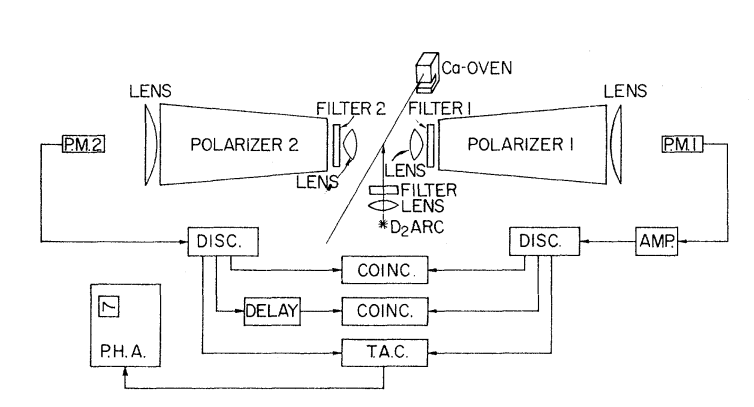
\includegraphics[width=\linewidth, height=0.7\textheight, keepaspectratio]{images/clauster.png}
        \caption{Scheme of the experimental setup \cite{Freedman1972}.}
      \end{figure}
    \end{column}
  \end{columns}

\end{frame}

% --- SLIDE 25: Results and Loopholes ---
\begin{frame}{Results, Verdict, and Loopholes}
  
  \begin{block}{Protocol and Result}
    \begin{itemize}[<+->]
      \item The experiment lasted approximately \textbf{200 hours} due to the low coincidence rate.
      \item A robust real-time normalization system was used to cancel out equipment drift.
    \end{itemize}
  \end{block}
  
  \begin{alertblock}<3->{The Decisive Experimental Result}
    \centering
    The measured value was:
    $\delta = 0.050 \pm 0.008$
  \end{alertblock}
  \pause

  \begin{block}<5->{Required Improvements: The Loopholes}
    \begin{itemize}[<+->]
      \item Despite its success, the experiment was not airtight:
      \begin{itemize}
          \item \textbf{Locality Loophole:} The polarizers could, in theory, ``communicate''. (Closed by Aspect in the 80s).
          \item \textbf{Detection Loophole:} The low efficiency could have biased the sample of detected pairs. (Closed in more recent experiments).
      \end{itemize}
    \end{itemize}
  \end{block}

\end{frame}
